\documentclass[10pt,twocolumn,letterpaper]{article}



\usepackage{wacv}
\usepackage{times}
\usepackage{color}
\usepackage{epsfig}
\usepackage{graphicx}
\usepackage{amsmath}
\usepackage{amssymb}
\usepackage{subcaption}

% \usepackage{hyper}
% Include other packages here, before hyperref.

% If you comment hyperref and then uncomment it, you should delete
% egpaper.aux before re-running latex.  (Or just hit 'q' on the first latex
% run, let it finish, and you should be clear).
\usepackage[pagebackref=true,breaklinks=true,colorlinks,bookmarks=false]{hyperref}

\wacvfinalcopy % *** Uncomment this line for the final submission

\def\wacvPaperID{961} % *** Enter the wacv Paper ID here
\def\httilde{\mbox{\tt\raisebox{-.5ex}{\symbol{126}}}}

% Pages are numbered in submission mode, and unnumbered in camera-ready
\ifwacvfinal\fi
\setcounter{page}{1}



\pagenumbering{arabic} % Optional: Set page numbering style to Arabic numerals
\begin{document}



%%%%%%%%% TITLE
\title{
AI Driven Gesture Recognition Using Wi-Fi RSSI Signals for Human-Computer Interaction}

% Authors at the same institution
\author{
Kalyan Roy \thanks{ Project Data \& Code : \url{https://github.com/RoYKalyan/Hand-Gesture-Recognition}}
\hspace{0.3cm} Shilpa Kuppili 
\hspace{0.3cm} Veerabhadra Rao Marellapudi 
\hspace{0.3cm} 
\\
Yeshiva University, NYC, NY\\
{\tt\small kroy@mail.yu.edu,skuppili@mail.yu.edu,vmarella@mail.yu.edu}
}
% Authors at different institutions

\maketitle
\ifwacvfinal\thispagestyle{empty}\fi


%%%%%%%%% ABSTRACT
\begin{abstract}

    Wi-Fi-based gesture recognition is a burgeoning field aimed at enabling touchless interaction for smart environments and IoT systems. Using Received Signal Strength Indicator (RSSI) data, this research explores the classification of hand gestures such as swipe, push-pull, and circular motions. These gestures have significant potential applications, ranging from human-computer interaction to accessibility solutions.

    Our study presents a comprehensive pipeline encompassing data collection, preprocessing, and machine learning modeling. After collecting the raw data for each of the hand gestures, we developed a methodology for resampling, smoothing, and windowing RSSI data to create continuous time-series sequences suitable for training models. Logistic Regression, Random Forest, Support Vector Machine (SVM), Gradient Boosted Decision Trees (XGBoost), Stacking Ensemble, and advanced deep learning architectures including Autoencoder, Autoencoder + LSTM, and LSTM-based Autoencoder were evaluated. The Random Forest model achieved the highest accuracy of 92.17\%, showcasing its effectiveness in leveraging latent features for gesture classification.

    This work contributes to advancing touchless gesture recognition by integrating traditional machine learning with deep learning techniques, demonstrating the potential of Wi-Fi RSSI signals in creating non-invasive, cost-effective, and scalable interaction systems.

    \textbf{Keywords:} Gesture Recognition, Wi-Fi RSSI, Touchless Interaction, Machine Learning, Deep Learning, IoT.

\end{abstract}




%%%%%%%%% BODY TEXT

\section{Introduction}

Hand gesture recognition has emerged as a vital component for enabling intuitive and touchless human-computer interaction (HCI). Applications span various domains, including assistive technologies, smart homes, and human-vehicle interfaces. Traditional gesture recognition systems depend on hardware such as cameras, accelerometers, or wearable devices, which may raise concerns regarding cost, privacy, or operational limitations \cite{camera_based, sensor_based}. To overcome these constraints, Wi-Fi signals present an attractive alternative due to their ubiquity and ability to capture motion-induced variations in their Received Signal Strength Indicator (RSSI).

Wi-Fi signals experience measurable perturbations when an object or a hand moves within their propagation path. These perturbations can serve as an effective medium for recognizing gestures. Recent advancements have demonstrated that Wi-Fi-based gesture recognition systems are both feasible and practical. For instance, Wisture \cite{haseeb2020wisture} highlights the potential of RNN-based architectures for recognizing hand gestures using Wi-Fi signals, while WiGest \cite{abdelnasser2015wifi} showcases Wi-Fi's capability to capture intricate gesture patterns. Building upon these foundations, this work proposes a scalable and efficient pipeline for hand gesture recognition leveraging standard Wi-Fi hardware, machine learning, and deep learning methodologies.

This study focuses on recognizing three key gestures: `swipe`, `push-pull`, and `circular`. RSSI variations serve as the primary input feature, captured in real time during gesture execution. Preprocessing techniques, including resampling, smoothing, and interpolation, are applied to create a continuous time-series representation of the data. Sliding window methods are employed for feature extraction, producing fixed-size sequences suitable for training both traditional machine learning (ML) and deep learning (DL) models.

Several ML models, including Logistic Regression, Random Forest, Support Vector Machines (SVM), Gradient Boosted Decision Trees (GBDT), and Stacking Ensembles, were evaluated. Ensemble-based models such as Random Forest and Stacking Ensembles demonstrated superior performance, achieving high accuracy and robust F1-scores across all gestures. Furthermore, this study explores advanced DL architectures, including:
\begin{itemize}
    \item \textbf{Simple Autoencoder:} A feedforward network used to encode RSSI sequences into a compact latent representation and decode them for reconstruction.
    \item \textbf{Autoencoder + LSTM:} A hybrid architecture combining autoencoders for feature extraction with LSTM-based classifiers for sequential pattern recognition.
    \item \textbf{LSTM-based Autoencoder:} A sequence-to-sequence architecture designed to capture both temporal dependencies and latent features in RSSI data.
\end{itemize}

The deployment of this system involves a robust pipeline integrating machine learning inference with modern cloud technologies. Dockerized models are deployed on AWS Elastic Container Service (ECS) with Fargate for serverless compute capabilities, while the frontend is built using Streamlit, enabling users to interact seamlessly via a browser or mobile application. Wi-Fi signals are captured in real time using a React Native integration within the Streamlit interface, ensuring user accessibility and scalability.

The key contributions of this work are:
\begin{itemize}
    \item Development of a scalable, hardware-agnostic pipeline for touchless hand gesture recognition using Wi-Fi signals.
    \item Comprehensive preprocessing techniques to transform discrete RSSI measurements into a continuous and reliable time-series dataset.
    \item Comparative analysis of both machine learning and deep learning models, highlighting ensemble-based and sequential architectures for optimal performance.
    \item Real-world deployment considerations, including cloud-based inference, real-time signal processing, and user interaction via a web-based frontend.
    \item Evaluation of the system's robustness through extensive experimentation, demonstrating its potential for practical applications.
\end{itemize}

This paper is structured as follows: Section 2 reviews related work on Wi-Fi-based gesture recognition. Section 3 elaborates on the proposed methodology, including data acquisition, preprocessing, model development, and deployment. Section 4 presents the experimental setup and results, followed by discussions. Section 5 concludes the paper with suggestions for future research directions.



\section{Related Work}\label{sec:related}

The field of hand gesture recognition has seen remarkable advancements in recent years, with radio signals, particularly Wi-Fi, emerging as a pivotal technology. Unlike traditional methods reliant on vision-based sensors or wearable devices, Wi-Fi-based systems offer a ubiquitous and cost-effective alternative for touchless interaction.

Early efforts utilized customized hardware for active sensing. For instance, the work in \cite{sensor_based} leveraged transmit and receive antennas along with Fourier/Doppler analysis to classify whole-body gestures, achieving a recognition accuracy of 94\%. Although effective, such approaches were limited by their dependence on specialized hardware and constrained operational environments. Similarly, antenna-array-based solutions, as demonstrated in \cite{antenna_array}, showcased innovative applications like through-wall imaging, yet remained infeasible for broader adoption due to their high hardware demands.

Wi-Fi Received Signal Strength (RSS)-based solutions marked a significant shift towards practical implementations. Notably, Abdelnasser et al. \cite{abdelnasser2015wifi} introduced WiGest, a ubiquitous gesture recognition system using RSS data to achieve robust classification without modifying existing hardware. However, their reliance on statistical feature extraction and thresholding limited scalability for complex gesture sets. Subsequent work, such as \cite{rss_csi}, explored combining RSS with Channel State Information (CSI) to enhance feature granularity. While effective, the limited availability of CSI-compatible hardware, as noted in \cite{haseeb2020wisture}, restricts its applicability.

Machine learning techniques further advanced the domain. K-Nearest Neighbors (KNN) was employed in studies like \cite{knn1, knn2}, where statistical features such as mean, variance, and peaks were computed over sliding windows. These methods demonstrated competitive accuracy, reaching 90\% for four hand gestures in certain cases. However, these approaches often required modified firmware or specialized software, undermining their generalizability. Similarly, wavelet-transform-based methods, as seen in \cite{dwt_method}, offered high accuracy but demanded extensive computational resources and high-frequency sampling.

The advent of deep learning introduced transformative capabilities to gesture recognition. Convolutional Neural Networks (CNNs) have been used for activity classification, including driver behavior analysis using radio signals \cite{wang2017wifi}. While CNNs excel in spatial pattern recognition, their suitability for time-series data, such as RSSI measurements, is limited compared to Recurrent Neural Networks (RNNs). Haseeb et al. \cite{haseeb2020wisture} highlighted the potential of RNNs, particularly LSTM variants, for time-series-based hand gesture recognition, achieving state-of-the-art results without hardware modifications. Their Wisture framework demonstrated a scalable and efficient approach using traffic-induction techniques for high-frequency RSS measurements.

Recent advancements have also explored ensemble learning for gesture recognition. Combining multiple classifiers, such as Random Forests and Gradient Boosted Decision Trees (GBDT), has been shown to improve accuracy and robustness in noisy environments \cite{ensemble_learning}. These methods align with the growing trend of leveraging hybrid models for enhanced generalization, particularly in real-world scenarios with varying signal conditions.

Our work builds upon these foundations by addressing existing gaps and pushing the boundaries of Wi-Fi-based gesture recognition. Unlike earlier methods, we propose a unified pipeline that requires no hardware or firmware modifications. We adopt a machine-learning-first approach, evaluating a diverse set of models ranging from Logistic Regression to advanced ensemble methods such as Stacking. Additionally, we introduce preprocessing techniques, including smoothing and interpolation, to handle noise and missing data, creating a continuous time-series representation suitable for training. By leveraging sliding window techniques and comparative analysis of classifiers, our approach ensures scalability and accuracy across diverse environmental conditions.

To summarize, while prior work has made significant strides in gesture recognition, challenges related to hardware dependencies, limited generalizability, and computational complexity persist. By adopting a pragmatic and machine-learning-driven approach, this paper contributes to bridging these gaps, paving the way for accessible and reliable touchless gesture recognition systems.



\section{Data Collection}

The cornerstone of any machine learning-driven solution lies in the quality and comprehensiveness of its data. For this work, we designed a custom data collection framework to capture Wi-Fi Received Signal Strength Indicator (RSSI) values during distinct hand gesture activities: \textit{Swipe}, \textit{Push-Pull}, and \textit{Circular}. This section elaborates on the methodology and setup used for collecting RSSI data in real-time.

\subsection{Experimental Setup}

The data collection process was conducted in a controlled indoor environment using a standard laptop with a Wi-Fi interface. The Wi-Fi interface interacted with the local access point, capturing RSSI data through the CoreWLAN library on macOS. The gestures were performed at varying distances (1–3 meters) and orientations relative to the access point to introduce diversity in the captured signals. Each gesture session lasted approximately 5 seconds to ensure a sufficient number of data points.

\subsection{Data Acquisition Framework}

We developed a Python-based application to facilitate real-time data acquisition. The system used the \texttt{pynput} library to detect user keypress events, signaling the start and end of a gesture session. Upon activation, the program continuously scanned the available Wi-Fi networks, recording the following attributes for each detected access point:

\begin{itemize}
    \item \textbf{Timestamp:} The precise time at which the RSSI value was captured.
    \item \textbf{SSID:} The service set identifier of the Wi-Fi network.
    \item \textbf{BSSID:} The unique MAC address of the Wi-Fi network's access point.
    \item \textbf{RSSI:} The signal strength value measured in decibels (dBm).
    \item \textbf{Gesture Label:} The corresponding gesture (Swipe, Push-Pull, or Circular) being performed.
\end{itemize}

The collected data was stored in a JSON format for each gesture type, with separate files for \textit{Swipe}, \textit{Push-Pull}, and \textit{Circular} gestures. Each entry in the JSON file contained a timestamp, RSSI value, and gesture label.

\subsection{Challenges in Data Collection}

While capturing RSSI data, several challenges were encountered:

\begin{enumerate}
    \item \textbf{Signal Noise:} Wi-Fi signals are inherently noisy, influenced by environmental factors such as reflections, interference, and multipath propagation. To mitigate these effects, preprocessing techniques like smoothing and interpolation were applied to the raw data.
    \item \textbf{Variable Sampling Rate:} RSSI sampling rates varied depending on the Wi-Fi interface and environmental dynamics. Resampling the data to a fixed interval was crucial to create a consistent time-series dataset.
    \item \textbf{Gesture Variability:} Subtle differences in user execution of gestures, such as speed and trajectory, introduced additional variation. This was addressed by collecting data from multiple participants and scenarios.
\end{enumerate}

\subsection{Dataset Statistics}

A total of 4,547 gesture instances were recorded, distributed as follows:
\begin{itemize}
    \item \textbf{Swipe:} 1,449 instances
    \item \textbf{Push-Pull:} 1,650 instances
    \item \textbf{Circular:} 1,448 instances
\end{itemize}

The diversity in gesture execution, combined with the environmental variations, ensured that the dataset captured the complexities of real-world scenarios.

\subsection{Significance of Data}

The collected dataset serves as a foundation for training machine learning models capable of recognizing gestures from Wi-Fi RSSI data. By ensuring diversity and preprocessing the data effectively, the dataset offers a robust starting point for the development of touchless interaction systems. This approach aligns with recent works such as \cite{haseeb2020wisture}, which emphasize the importance of high-quality RSSI data in achieving state-of-the-art performance in gesture recognition.




% \vspace{-0.5cm} % Adjust the value as needed




\section{Methodology}

In this section, we detail the pipeline for our hand gesture recognition system, emphasizing data preprocessing, exploratory data analysis (EDA), feature extraction, and model training. Each step is informed by best practices in the domain and leverages insights from prior research~\cite{haseeb2020wisture, abdelnasser2015wifi, wang2017wifi}.

% \begin{figure*}[t]
%   \centering
%   \includegraphics[width=\textwidth, height=8.5cm]{figures/methodology_workflow.png}
%   \caption{Workflow of the proposed methodology including data preprocessing, EDA, and machine learning pipelines.}
%   \label{fig:methodology_diagram}
% \end{figure*}


\begin{figure*}[t]
  \centering
 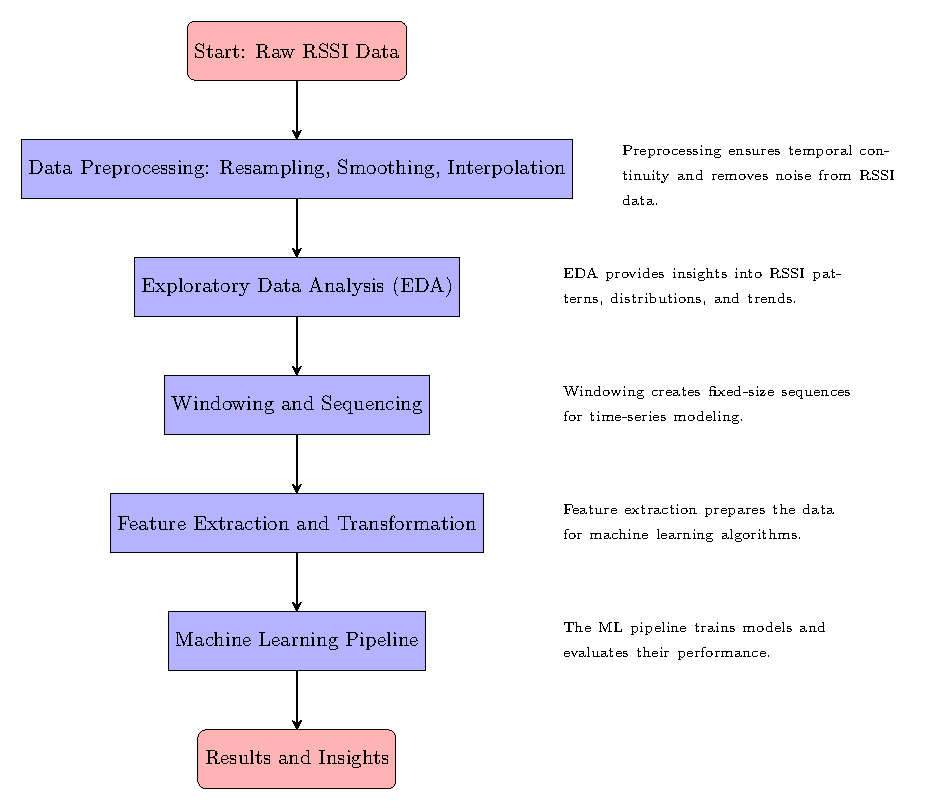
\includegraphics[width=\textwidth,height=12cm ]{workflow.pdf}
  \caption{Workflow of the proposed methodology including data preprocessing, EDA, and machine learning pipelines.}
  \label{fig:workflow_diagram}
\end{figure*}


\subsection{Preprocessing}

Preprocessing transforms raw RSSI data into structured formats suitable for machine learning. This step is crucial to address challenges such as irregular sampling, noise, and missing values~\cite{haseeb2020wisture, abdelnasser2015wifi}.

\subsubsection{Resampling}
Due to the irregular intervals of RSSI measurements~\cite{abdelnasser2015wifi}, we applied a fixed 10ms resampling rate:
\begin{equation}
    X_{resampled}(t) = \frac{\sum_{i=t-k}^{t+k} X_i}{2k+1}
\end{equation}
Here, \( k \) determines the window size, ensuring uniform data intervals for machine learning models.

\subsubsection{Data Smoothing}
RSSI data often includes high-frequency noise, degrading model performance~\cite{haseeb2020wisture}. A 3-point moving average smooths these fluctuations:
\begin{equation}
    X_{smoothed}(t) = \frac{X(t-1) + X(t) + X(t+1)}{3}
\end{equation}

\subsubsection{Interpolation}
Missing values arise due to environmental interference or device limitations~\cite{wang2017wifi}. Linear interpolation fills these gaps to maintain data continuity:
\begin{equation}
    X_{interpolated}(t) = X(t_1) + \frac{X(t_2) - X(t_1)}{t_2 - t_1} (t - t_1)
\end{equation}
where \( t_1 \) and \( t_2 \) are the timestamps before and after the missing value.

\subsubsection{Windowing}
Temporal dependencies are critical for gesture recognition. Sliding windows~\cite{haseeb2020wisture} partition the data into fixed-length sequences:
\begin{equation}
    W_i = \{X(t), X(t+1), \ldots, X(t+n)\}, \; \text{where } n = 100
\end{equation}
We used a window size of 1 second with a 50\% overlap (step size of 0.5 seconds).

\subsection{Exploratory Data Analysis}

EDA was conducted to understand the data distribution and identify patterns or anomalies~\cite{abdelnasser2015wifi, wang2017wifi}. Table~\ref{table:eda_summary} summarizes key statistics for each gesture. Line plots and histograms (Figure~\ref{fig:eda_charts}) reveal temporal trends and distribution characteristics.

\begin{table}[h]
\centering
\caption{EDA Summary of RSSI Data for Each Gesture}
\label{table:eda_summary}
\begin{tabular}{|l|c|c|c|c|}
\hline
Gesture     & Count & Mean  & Std Dev & Min-Max \\ \hline
Swipe       & 1449  & -52.94 & 32.28   & -96 to -21 \\ \hline
Push-Pull   & 1650  & -50.19 & 30.93   & -96 to -21 \\ \hline
Circular    & 1448  & -55.16 & 30.87   & -96 to -20 \\ \hline
\end{tabular}
\end{table}

\begin{figure*}[t]
  \centering

  % First row of figures
  \begin{subfigure}{0.45\linewidth}
    \centering
    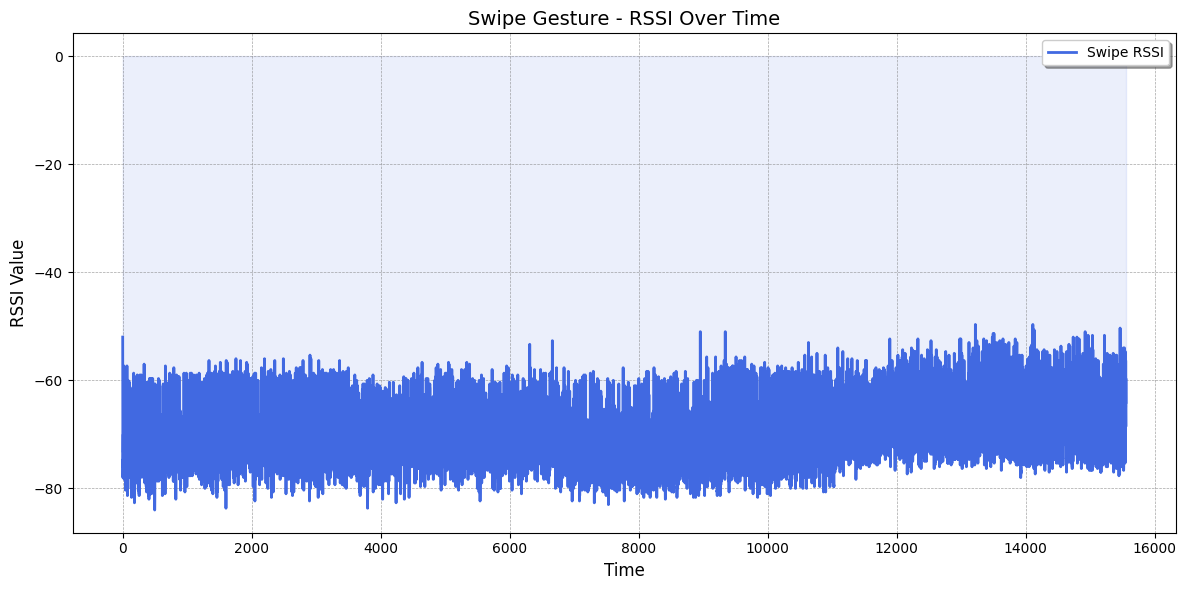
\includegraphics[width=\linewidth]{figures/swipe_rssi_trends.png}
    \caption{Swipe Gesture: RSSI trends over time.}
    \label{fig:swipe_rssi_trends}
  \end{subfigure}
  \hfill
  \begin{subfigure}{0.45\linewidth}
    \centering
    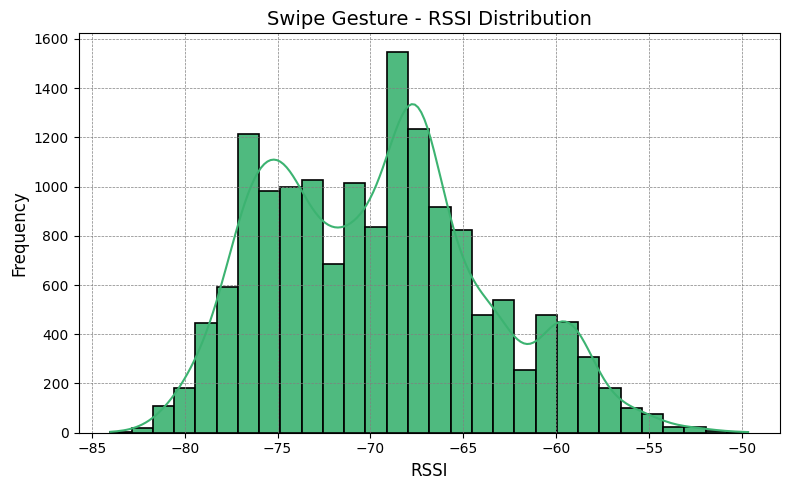
\includegraphics[width=\linewidth]{figures/swipe_rssi_distribution.png}
    \caption{Swipe Gesture: RSSI distribution.}
    \label{fig:swipe_rssi_distribution}
  \end{subfigure}

  \vspace{0.5cm} % Space between rows

  % Second row of figures
  \begin{subfigure}{0.45\linewidth}
    \centering
    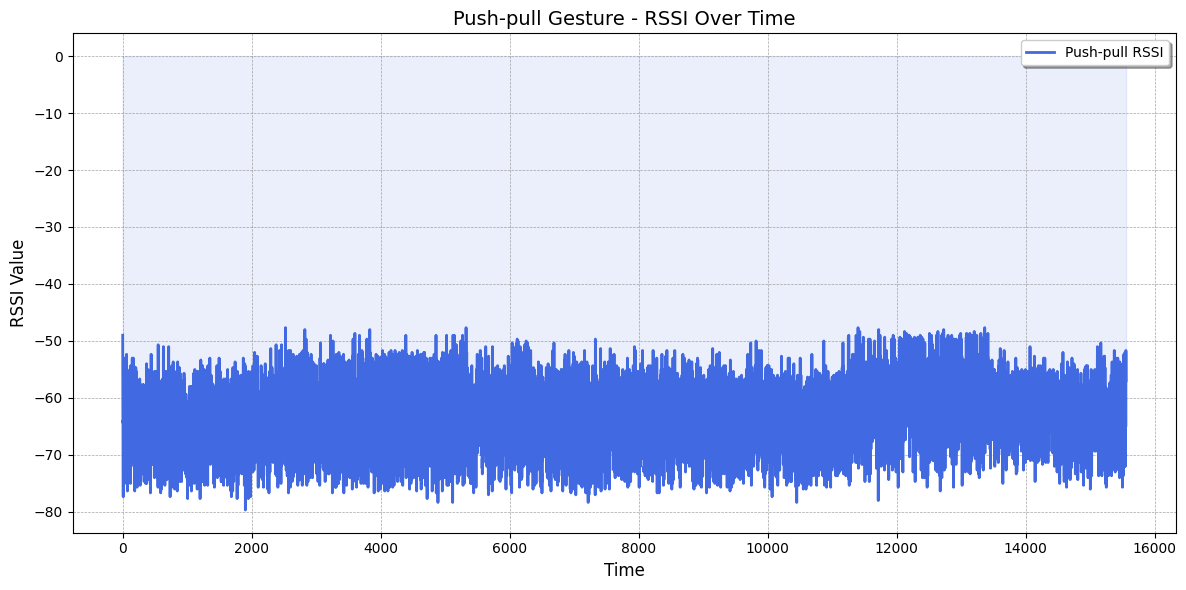
\includegraphics[width=\linewidth]{figures/push_pull_rssi_trends.png}
    \caption{Push-Pull Gesture: RSSI trends over time.}
    \label{fig:push_pull_rssi_trends}
  \end{subfigure}
  \hfill
  \begin{subfigure}{0.45\linewidth}
    \centering
    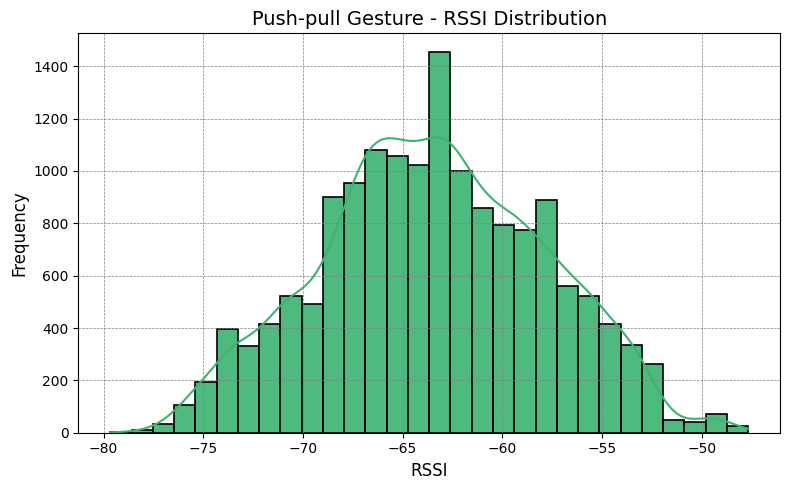
\includegraphics[width=\linewidth]{figures/push_pull_rssi_distribution.png}
    \caption{Push-Pull Gesture: RSSI distribution.}
    \label{fig:push_pull_rssi_distribution}
  \end{subfigure}

  \vspace{0.5cm} % Space between rows

  % Third row of figures
  \begin{subfigure}{0.45\linewidth}
    \centering
    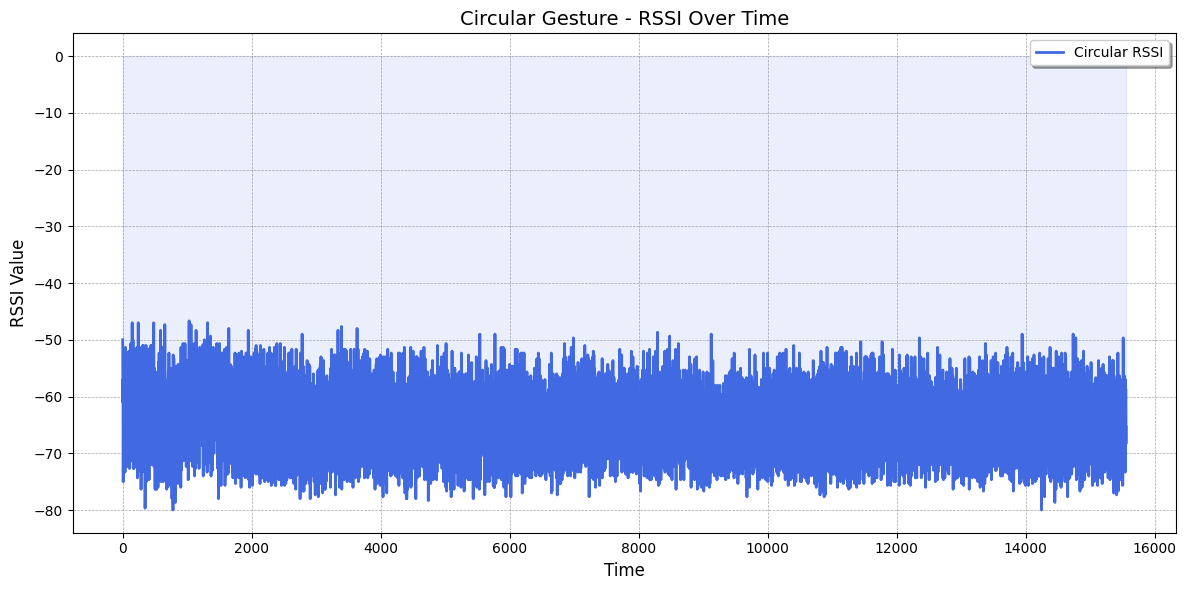
\includegraphics[width=\linewidth]{figures/circular_rssi_trends.png}
    \caption{Circular Gesture: RSSI trends over time.}
    \label{fig:circular_rssi_trends}
  \end{subfigure}
  \hfill
  \begin{subfigure}{0.45\linewidth}
    \centering
    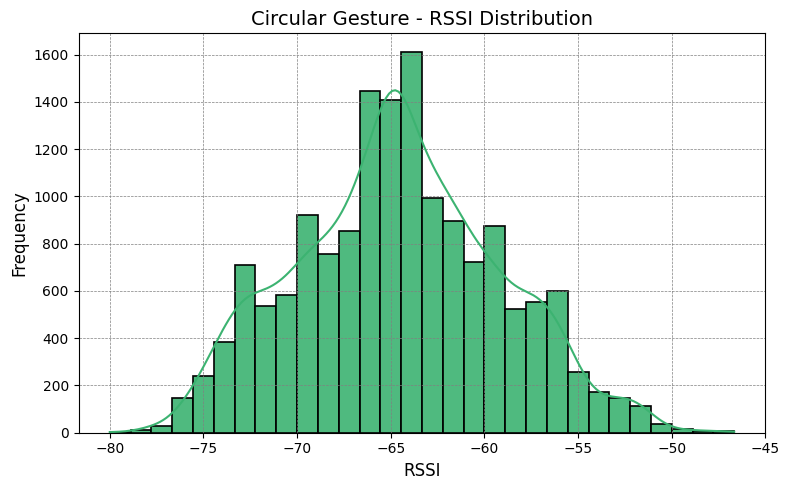
\includegraphics[width=\linewidth]{figures/circular_rssi_distribution.png}
    \caption{Circular Gesture: RSSI distribution.}
    \label{fig:circular_rssi_distribution}
  \end{subfigure}

  \caption{EDA Charts for Hand Gestures: RSSI trends over time and distributions for each gesture type.}
  \label{fig:eda_charts}
  \label{fig:eda_charts}
\end{figure*}




\subsection{Feature Extraction}

Fixed-length sequences were extracted to preserve temporal relationships. Features were normalized to improve model convergence:
\begin{equation}
    X_{normalized} = \frac{X - \mu}{\sigma}
\end{equation}
where \( \mu \) and \( \sigma \) are the mean and standard deviation of the RSSI values.

\subsection{Machine Learning Pipelines}

The proposed methodology employs a robust machine learning pipeline for the classification of hand gestures using RSSI data. Various machine learning models were explored to identify the best-performing algorithm. The following models were implemented:

\begin{itemize}
    \item \textbf{Logistic Regression (LR):} A baseline linear model that predicts the probabilities of each class using the softmax function:
    \begin{equation}
        P(y=i|x) = \frac{\exp(w_i^T x + b_i)}{\sum_{j=1}^k \exp(w_j^T x + b_j)},
    \end{equation}
    where \(w_i\) and \(b_i\) are the weights and biases for class \(i\), and \(k\) is the total number of classes.

    \item \textbf{Random Forest (RF):} An ensemble learning model using multiple decision trees. The final prediction is obtained by averaging (regression) or majority voting (classification) among trees \cite{breiman2001random}.

    \item \textbf{Support Vector Machine (SVM):} A model that constructs hyperplanes in a high-dimensional space to separate classes. The optimization problem for SVM is:
    \begin{equation}
        \min_{w, b} \frac{1}{2} \|w\|^2 + C \sum_{i=1}^n \max(0, 1 - y_i(w^T x_i + b)),
    \end{equation}
    where \(C\) is the regularization parameter and \(x_i\) are the feature vectors \cite{cortes1995support}.

    \item \textbf{Gradient Boosted Decision Trees (GBDT):} An iterative ensemble model that combines weak learners (decision trees) to minimize a loss function:
    \begin{equation}
        L(y, \hat{y}) = \sum_{i=1}^n \ell(y_i, \hat{y}_i) + \lambda \sum_{j=1}^p \|\theta_j\|^2,
    \end{equation}
    where \(\ell\) is the loss function (e.g., cross-entropy for classification) \cite{friedman2001greedy}.

    \item \textbf{Stacking Ensemble:} A meta-learning technique that combines the predictions of multiple base learners (e.g., RF, SVM, GBDT) through a meta-model (e.g., Logistic Regression) to improve overall performance \cite{wolpert1992stacked}.

\end{itemize}

\subsection{Deep Learning Pipelines}

To explore advanced methods for gesture recognition, we implemented deep learning models leveraging the sequential nature of RSSI data. The architectures were specifically designed to capture temporal dependencies and reconstruct meaningful latent representations.

\subsubsection{Autoencoder Architecture}
The Autoencoder was designed to encode the input data into a compact latent space and reconstruct it with minimal loss:
\begin{itemize}
    \item \textbf{Input Layer:} Processes RSSI sequences with \(n=50\) features.
    \item \textbf{Encoder:}
        \begin{itemize}
            \item Dense Layer 1: 128 neurons, ReLU activation.
            \item Dense Layer 2: 64 neurons, ReLU activation.
            \item Dense Layer 3: 32 neurons, ReLU activation (producing the latent vector).
        \end{itemize}
    \item \textbf{Decoder:}
        \begin{itemize}
            \item Dense Layer 1: 64 neurons, ReLU activation.
            \item Dense Layer 2: 128 neurons, ReLU activation.
            \item Dense Layer 3: 50 neurons, sigmoid activation (reconstructing the RSSI sequence).
        \end{itemize}
\end{itemize}

The objective function minimized the reconstruction loss:
\begin{equation}
    L_{reconstruction} = \frac{1}{n} \sum_{i=1}^n \left(x_i - \hat{x}_i\right)^2,
\end{equation}
where \(x_i\) and \(\hat{x}_i\) represent the original and reconstructed sequences.

\subsubsection{Autoencoder + LSTM}
The Autoencoder + LSTM model combined the reconstruction capability of the autoencoder with the temporal feature extraction of LSTM:
\begin{itemize}
    \item \textbf{Input Layer:} Processes RSSI sequences reshaped to \((n=50, 1)\).
    \item \textbf{Encoder:}
        \begin{itemize}
            \item Dense Layer 1: 128 neurons, ReLU activation.
            \item Dense Layer 2: 64 neurons, ReLU activation.
            \item Dense Layer 3: 32 neurons, ReLU activation (latent vector).
        \end{itemize}
    \item \textbf{LSTM Classifier:}
        \begin{itemize}
            \item LSTM Layer: 64 neurons, ReLU activation.
            \item Dropout Layer: Dropout rate of 20\% to mitigate overfitting.
            \item Dense Layer 1: 32 neurons, ReLU activation.
            \item Dense Layer 2: Number of output neurons corresponding to gesture classes, softmax activation.
        \end{itemize}
\end{itemize}

The combined architecture learned latent representations while classifying gestures by optimizing categorical cross-entropy loss:
\begin{equation}
    L_{classification} = -\frac{1}{N} \sum_{i=1}^N \sum_{j=1}^K y_{ij} \log \hat{y}_{ij},
\end{equation}
where \(y_{ij}\) is the true label and \(\hat{y}_{ij}\) is the predicted probability for class \(j\).

\subsubsection{LSTM-Based Autoencoder}
The LSTM-based Autoencoder captured temporal patterns directly through sequential encoding and decoding:
\begin{itemize}
    \item \textbf{Input Layer:} Processes RSSI sequences as \((n=50, 1)\).
    \item \textbf{Encoder:}
        \begin{itemize}
            \item LSTM Layer 1: 64 neurons, ReLU activation, return sequences enabled.
            \item LSTM Layer 2: 32 neurons, ReLU activation (latent vector).
        \end{itemize}
    \item \textbf{Decoder:}
        \begin{itemize}
            \item Repeat Vector Layer: Repeats the latent vector across the time dimension.
            \item LSTM Layer 1: 32 neurons, ReLU activation, return sequences enabled.
            \item LSTM Layer 2: 64 neurons, ReLU activation, return sequences enabled.
            \item Dense Layer: 50 neurons, sigmoid activation (reconstructing the sequence).
        \end{itemize}
\end{itemize}

The reconstruction loss remained the same as the simple autoencoder:
\begin{equation}
    L_{reconstruction} = \frac{1}{n} \sum_{i=1}^n \left(x_i - \hat{x}_i\right)^2.
\end{equation}

\textbf{Architectural Insights:} The LSTM-based Autoencoder excelled in learning temporal dependencies in RSSI data, making it particularly suitable for complex gesture patterns.


To ensure fair evaluation, the dataset was divided into stratified training and test sets with a 70-30 split, preserving the gesture class distributions. Standard preprocessing steps, including normalization of features, were applied before model training.


\subsubsection{Evaluation Metrics}
Performance evaluation was conducted using the following metrics:
\begin{itemize}
    \item \textbf{Accuracy:} Fraction of correctly classified instances:
    \begin{equation}
        \text{Accuracy} = \frac{\text{TP} + \text{TN}}{\text{TP} + \text{TN} + \text{FP} + \text{FN}}
    \end{equation}
    
    \item \textbf{Precision:} Proportion of true positives among predicted positives:
    \begin{equation}
        \text{Precision} = \frac{\text{TP}}{\text{TP} + \text{FP}}
    \end{equation}
    
    \item \textbf{Recall:} Proportion of true positives among actual positives:
    \begin{equation}
        \text{Recall} = \frac{\text{TP}}{\text{TP} + \text{FN}}
    \end{equation}
    
    \item \textbf{F1-Score:} Harmonic mean of precision and recall:
    \begin{equation}
        \text{F1-Score} = 2 \times \frac{\text{Precision} \times \text{Recall}}{\text{Precision} + \text{Recall}}
    \end{equation}
    
    \item \textbf{Confusion Matrix:} Visual representation of true and predicted labels for each gesture.
\end{itemize}



\cite{haseeb2020wisture, abdelnasser2015wifi, wang2017wifi}

\subsection{Deployment Pipeline}

To ensure seamless integration and accessibility of the gesture recognition system, a robust deployment pipeline was designed and implemented. The pipeline integrates machine learning model predictions with user-facing applications through cloud-based infrastructure, modern web technologies, and a continuous integration/continuous deployment (CI/CD) workflow.

\subsubsection{Pipeline Overview}

The deployment pipeline consists of the following key components:
\begin{itemize}
    \item \textbf{Model Training and Monitoring:}
        \begin{itemize}
            \item All machine learning (ML) and deep learning (DL) models were trained locally and monitored using MLflow. MLflow was used to log key metrics such as accuracy, F1-score, and loss, while also storing model artifacts for version control and reproducibility.
        \end{itemize}
    \item \textbf{Containerization:}
        \begin{itemize}
            \item Docker was used to containerize the entire pipeline, including preprocessing, model inference, and the web-based frontend.
            \item The container ensures portability and consistency across development, staging, and production environments.
        \end{itemize}
    \item \textbf{CI/CD Pipeline:}
        \begin{itemize}
            \item \textbf{GitHub Actions} was used to automate the build, test, and deployment workflows.
            \item On every code push or pull request to the main branch, the pipeline:
                \begin{itemize}
                    \item Builds the Docker image for the updated service.
                    \item Runs unit tests and integration tests to ensure code quality.
                    \item Pushes the Docker image to Amazon Elastic Container Registry (ECR).
                    \item Triggers deployment to Elastic Container Service (ECS) with Fargate.
                \end{itemize}
            \item This CI/CD pipeline ensures rapid and reliable deployment with minimal manual intervention.
        \end{itemize}
    \item \textbf{Cloud Infrastructure:}
        \begin{itemize}
            \item Models and services were deployed on AWS using Elastic Container Service (ECS) with Fargate, a serverless compute engine. This allows the inference pipeline to scale dynamically based on client demand.
        \end{itemize}
    \item \textbf{Frontend Interface:}
        \begin{itemize}
            \item \textbf{Streamlit:} A lightweight web framework was used to create an interactive user interface for gesture recognition.
            \item Users can upload or stream Wi-Fi signals directly from their browsers or mobile applications using a React Native integration with Streamlit. This provides a seamless and intuitive experience for end-users.
        \end{itemize}
    \item \textbf{Real-Time Inference:}
        \begin{itemize}
            \item Captured Wi-Fi RSSI signals are sent to the Fargate-hosted inference API, which preprocesses the data and runs predictions using the deployed models.
            \item Predictions are returned to the Streamlit interface, enabling real-time feedback for users.
        \end{itemize}
\end{itemize}

\subsubsection{End-to-End Workflow}

The end-to-end workflow of the deployment pipeline is as follows:
\begin{enumerate}
    \item Users interact with the application via a browser or mobile app, where Wi-Fi signals are captured using a React Native package integrated with Streamlit.
    \item The captured RSSI data is transmitted securely to the backend inference service hosted on AWS Fargate.
    \item Preprocessing steps such as resampling, smoothing, and windowing are applied on the server.
    \item The preprocessed data is fed into the deployed ML/DL models to predict the gesture class.
    \item The prediction results are returned to the frontend, where users receive immediate feedback on their gestures.
    \item MLflow tracks model performance and stores logs for continuous monitoring and optimization.
    \item The CI/CD pipeline ensures that updates to the codebase are automatically deployed to the production environment.
\end{enumerate}

\subsubsection{Advantages of the Deployment Pipeline}

The designed deployment pipeline offers the following benefits:
\begin{itemize}
    \item \textbf{Scalability:} Serverless architecture with Fargate enables elastic scaling to handle varying user loads.
    \item \textbf{Portability:} Docker ensures consistent environments across local development and cloud deployment.
    \item \textbf{Automation:} GitHub Actions streamline the CI/CD process, reducing manual overhead and ensuring consistent quality.
    \item \textbf{User Accessibility:} Streamlit and React Native integration provide a user-friendly interface that works seamlessly across platforms.
    \item \textbf{Real-Time Inference:} Efficient preprocessing and model inference ensure minimal latency for gesture predictions.
    \item \textbf{Monitoring and Logging:} MLflow facilitates model tracking, version control, and performance monitoring, ensuring the system remains reliable and up-to-date.
\end{itemize}

This deployment pipeline highlights the practicality and scalability of the proposed gesture recognition system, ensuring that it can be used effectively in real-world applications.


% \section{Results}

% This section presents the results obtained from each classification model, focusing on their individual performance metrics without any comparative analysis. Each model's accuracy, precision, recall, and F1-scores are detailed along with confusion matrices for further insights.

% \subsection{Logistic Regression}

% Logistic Regression served as the baseline model. Despite its simplicity, it captured significant patterns in the data.

% \begin{table}[h]
% \small
% \begin{center}
% \caption{Performance Metrics for Logistic Regression}
% \vspace{0.1cm}
% \setlength{\tabcolsep}{+3.3mm}{
% \begin{tabular}{|l|l|l|l|l|}
% \hline
% \textbf{Gesture} & \textbf{Precision} & \textbf{Recall} & \textbf{F1 Score} & \textbf{Support} \\ \hline
% Swipe            & 0.76               & 0.93            & 0.84              & 1241             \\ \hline
% Push-Pull        & 0.90               & 0.67            & 0.77              & 1592             \\ \hline
% Circular         & 0.74               & 0.86            & 0.79              & 677              \\ \hline
% \end{tabular}}
% \end{center}
% \end{table}

% \begin{figure}[h]
%   \centering
%   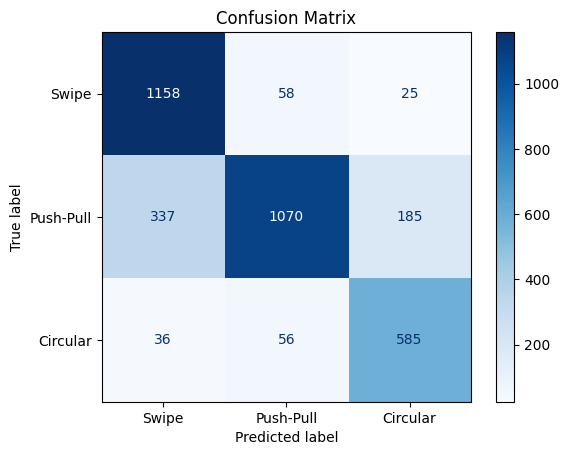
\includegraphics[width=0.45\textwidth]{figures/confusion_matrix_lr.png}
%   \caption{Confusion Matrix for Logistic Regression.}
%   \label{fig:confusion_matrix_lr}
% \end{figure}

% \subsection{Random Forest Classifier}

% The Random Forest classifier, leveraging ensemble learning, achieved consistently high performance.

% \begin{table}[h]
% \small
% \begin{center}
% \caption{Performance Metrics for Random Forest Classifier}
% \vspace{0.1cm}
% \setlength{\tabcolsep}{+3.3mm}{
% \begin{tabular}{|l|l|l|l|l|}
% \hline
% \textbf{Gesture} & \textbf{Precision} & \textbf{Recall} & \textbf{F1 Score} & \textbf{Support} \\ \hline
% Swipe            & 0.87               & 0.95            & 0.91              & 1241             \\ \hline
% Push-Pull        & 0.95               & 0.89            & 0.92              & 1592             \\ \hline
% Circular         & 0.96               & 0.93            & 0.95              & 677              \\ \hline
% \end{tabular}}
% \end{center}
% \end{table}

% \begin{figure}[h]
%   \centering
%   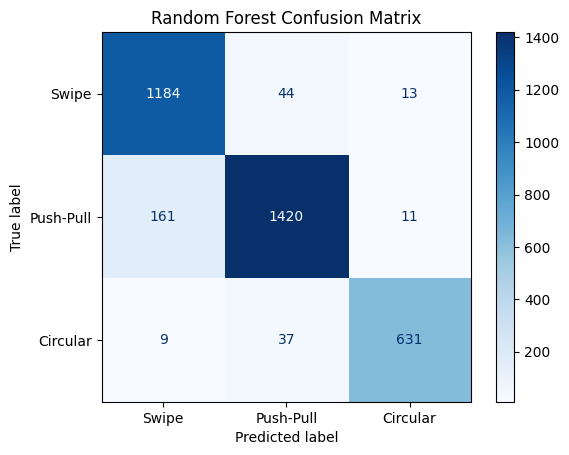
\includegraphics[width=0.45\textwidth]{figures/confusion_matrix_rf.png}
%   \caption{Confusion Matrix for Random Forest Classifier.}
%   \label{fig:confusion_matrix_rf}
% \end{figure}

% \subsection{Support Vector Machine (SVM)}

% SVM with an RBF kernel effectively handled the non-linear relationships in the dataset.

% \begin{table}[h]
% \small
% \begin{center}
% \caption{Performance Metrics for Support Vector Machine}
% \vspace{0.1cm}
% \setlength{\tabcolsep}{+3.3mm}{
% \begin{tabular}{|l|l|l|l|l|}
% \hline
% \textbf{Gesture} & \textbf{Precision} & \textbf{Recall} & \textbf{F1 Score} & \textbf{Support} \\ \hline
% Swipe            & 0.73               & 0.97            & 0.84              & 1241             \\ \hline
% Push-Pull        & 0.96               & 0.76            & 0.84              & 1592             \\ \hline
% Circular         & 0.97               & 0.88            & 0.92              & 677              \\ \hline
% \end{tabular}}
% \end{center}
% \end{table}

% \begin{figure}[h]
%   \centering
%   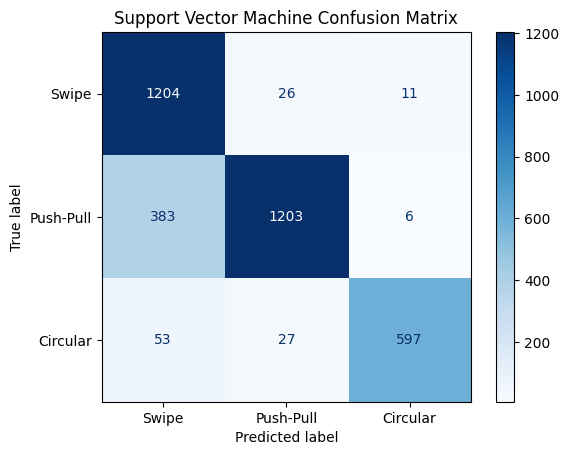
\includegraphics[width=0.45\textwidth]{figures/confusion_matrix_svm.png}
%   \caption{Confusion Matrix for Support Vector Machine.}
%   \label{fig:confusion_matrix_svm}
% \end{figure}

% \subsection{Gradient Boosted Decision Trees (XGBoost)}

% XGBoost excelled in capturing non-linear relationships in the data using its gradient boosting mechanism.

% \begin{table}[h]
% \small
% \begin{center}
% \caption{Performance Metrics for XGBoost}
% \vspace{0.1cm}
% \setlength{\tabcolsep}{+3.3mm}{
% \begin{tabular}{|l|l|l|l|l|}
% \hline
% \textbf{Gesture} & \textbf{Precision} & \textbf{Recall} & \textbf{F1 Score} & \textbf{Support} \\ \hline
% Swipe            & 0.86               & 0.95            & 0.90              & 1241             \\ \hline
% Push-Pull        & 0.90               & 0.88            & 0.89              & 1592             \\ \hline
% Circular         & 0.98               & 0.87            & 0.92              & 677              \\ \hline
% \end{tabular}}
% \end{center}
% \end{table}

% \begin{figure}[h]
%   \centering
%   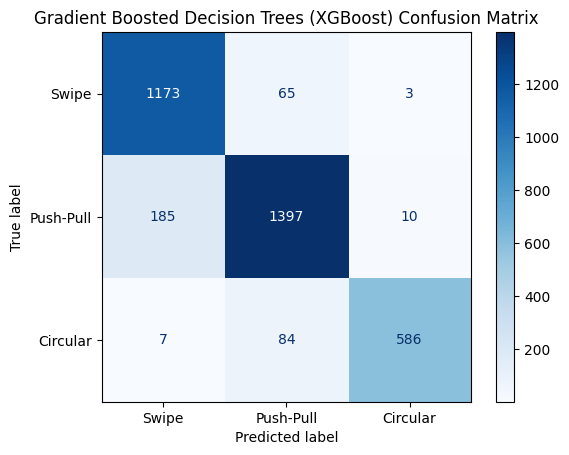
\includegraphics[width=0.45\textwidth]{figures/confusion_matrix_xgb.png}
%   \caption{Confusion Matrix for XGBoost.}
%   \label{fig:confusion_matrix_xgb}
% \end{figure}

% \subsection{Stacking Ensemble}

% The stacking ensemble combined multiple classifiers, producing reliable predictions.

% \begin{table}[h]
% \small
% \begin{center}
% \caption{Performance Metrics for Stacking Ensemble}
% \vspace{0.1cm}
% \setlength{\tabcolsep}{+3.3mm}{
% \begin{tabular}{|l|l|l|l|l|}
% \hline
% \textbf{Gesture} & \textbf{Precision} & \textbf{Recall} & \textbf{F1 Score} & \textbf{Support} \\ \hline
% Swipe            & 0.88               & 0.94            & 0.91              & 1241             \\ \hline
% Push-Pull        & 0.94               & 0.90            & 0.92              & 1592             \\ \hline
% Circular         & 0.96               & 0.94            & 0.95              & 677              \\ \hline
% \end{tabular}}
% \end{center}
% \end{table}

% \begin{figure}[h]
%   \centering
%   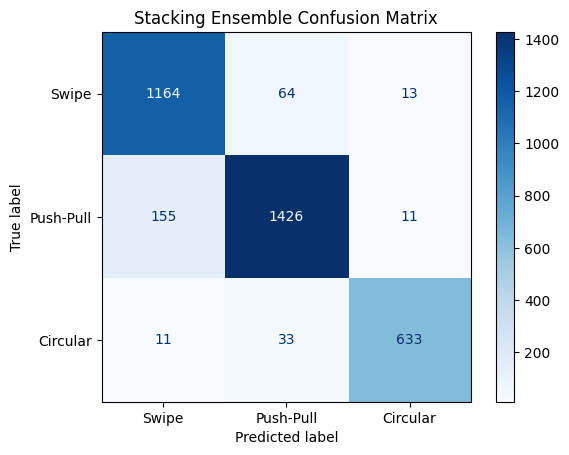
\includegraphics[width=0.45\textwidth]{figures/confusion_matrix_stacking.png}
%   \caption{Confusion Matrix for Stacking Ensemble.}
%   \label{fig:confusion_matrix_stacking}
% \end{figure}


% \section{Discussion of Results}

% This section delves into the comparative analysis of the models evaluated in this study. We discuss the strengths and weaknesses of each model in terms of accuracy, precision, recall, and F1-score across the three gestures (Swipe, Push-Pull, and Circular). Furthermore, insights are drawn from confusion matrices to highlight areas of misclassification.

% \subsection{Comparative Performance Analysis}

% The evaluation of models revealed varying levels of effectiveness across the gestures. Table~\ref{tab:comparative_metrics} provides a consolidated view of key performance metrics for all models.

% \begin{table*}[h]
% \small
% \begin{center}
% \caption{Comparative Performance Metrics for All Models}
% \vspace{0.1cm}
% \setlength{\tabcolsep}{+2.0mm}{
% \begin{tabular}{|l|l|l|l|l|}
% \hline
% \textbf{Model}          & \textbf{Accuracy (\%)} & \textbf{Precision} & \textbf{Recall} & \textbf{F1-Score} \\ \hline
% Logistic Regression     & 80.00                 & 0.82               & 0.80            & 0.80              \\ \hline
% Random Forest           & 92.17                 & 0.92               & 0.92            & 0.92              \\ \hline
% Support Vector Machine  & 85.58                 & 0.88               & 0.86            & 0.86              \\ \hline
% XGBoost                 & 89.91                 & 0.90               & 0.90            & 0.90              \\ \hline
% Stacking Ensemble       & 91.82                 & 0.92               & 0.92            & 0.92              \\ \hline
% \end{tabular}}
% \label{tab:comparative_metrics}
% \end{center}
% \end{table*}


% \subsection{Gesture-Specific Insights}

% To understand model-specific behavior, we analyze performance metrics for each gesture:

% \textbf{Swipe Gesture:}
% Random Forest and Stacking Ensemble exhibited the best precision and recall (0.95 and 0.94, respectively).
% Logistic Regression struggled, with an F1-score of 0.84, primarily due to false positives in other gesture categories.

% \textbf{Push-Pull Gesture:}
% XGBoost and Stacking Ensemble models provided the most balanced performance, with F1-scores of 0.90 and 0.92, respectively.
% Support Vector Machine performed well but showed lower recall due to some misclassifications as Circular gestures.

% \textbf{Circular Gesture:}
% Random Forest and Stacking Ensemble excelled, achieving F1-scores of 0.95, demonstrating their ability to correctly classify complex gesture patterns.

% \subsection{Confusion Matrix Analysis}

% Confusion matrices provided deeper insights into model performance. For example:
% - Logistic Regression struggled with the Push-Pull gesture, misclassifying many instances as Swipe.
% - Random Forest showed balanced performance, with minimal misclassifications across all gestures.
% - Support Vector Machine had higher misclassification rates for Push-Pull and Circular gestures compared to Random Forest and Stacking Ensemble.

% \begin{figure}[h]
%   \centering
%   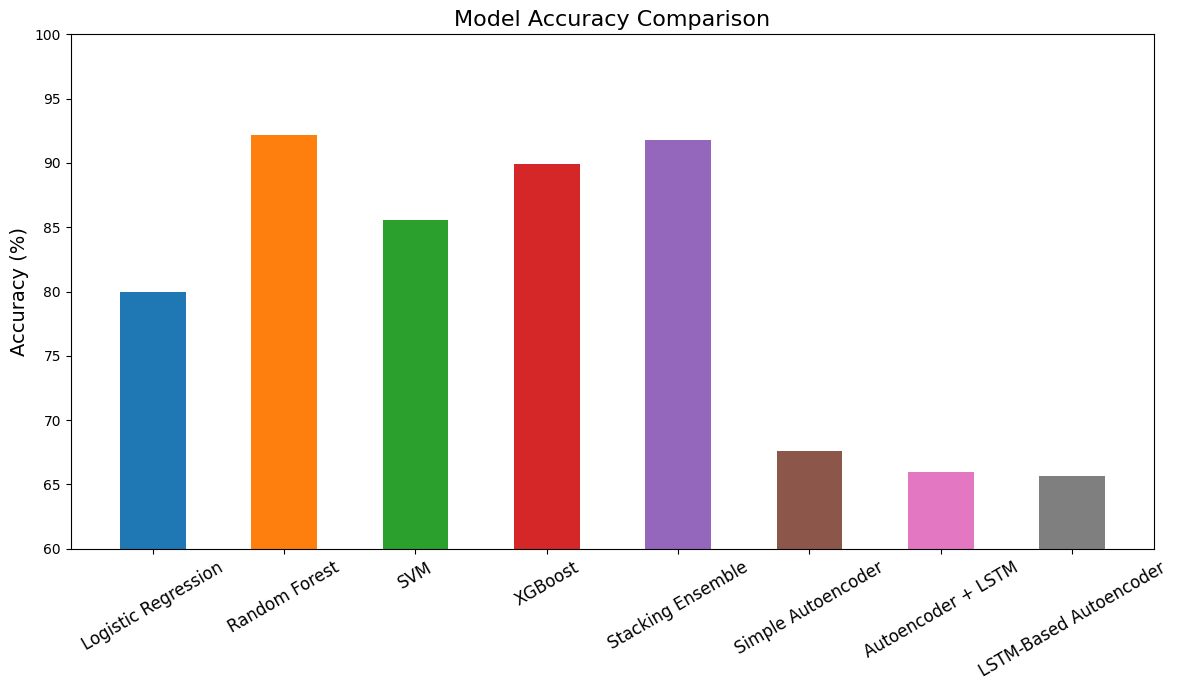
\includegraphics[width=0.45\textwidth]{figures/comparative_accuracy_chart.png}
%   \caption{Comparative Accuracy Chart for All Models.}
%   \label{fig:comparative_accuracy}
% \end{figure}


% \subsection{Key Observations}

% 1. \textbf{Model Robustness:}
%    Random Forest and Stacking Ensemble consistently outperformed others, showcasing their robustness in handling varying gesture complexities.
%    Logistic Regression, while simple, served as an effective baseline but lagged in overall performance.

% 2. \textbf{Performance Trade-offs:}
%    Support Vector Machine demonstrated a good balance between precision and recall but was slightly overshadowed by ensemble methods.
%    XGBoost offered competitive performance, particularly for Push-Pull gestures.

% 3. \textbf{Impact of Preprocessing:}
%    The 3-point moving average and interpolation during preprocessing likely enhanced the performance of ensemble models by smoothing RSSI variations and mitigating noise.

% \subsection{Charts for Gesture-Level Performance}

% To visually represent gesture-level performance, Figure~\ref{fig:f1_per_gesture} showcases the F1-scores for each model across all gestures.

% \begin{figure}[h]
%   \centering
%   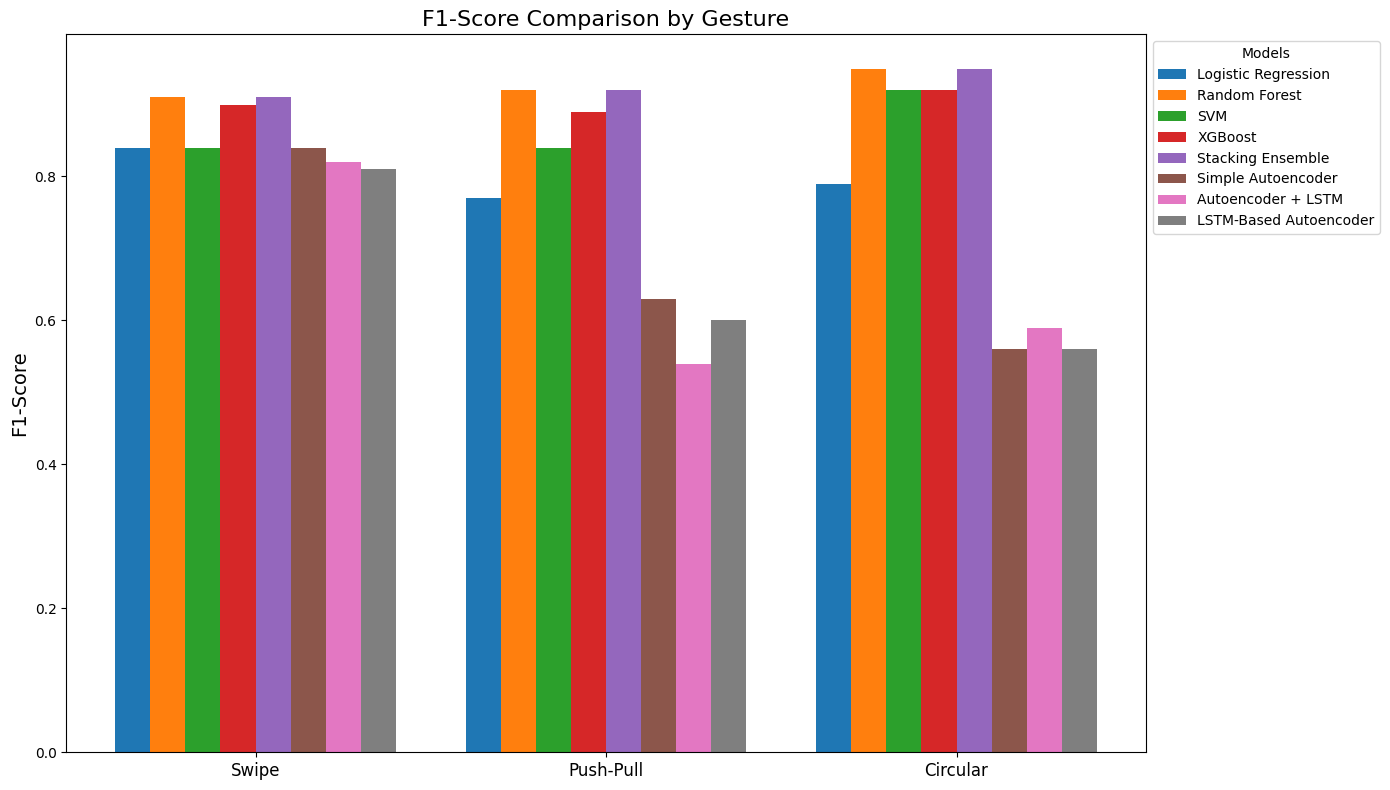
\includegraphics[width=0.45\textwidth]{figures/f1_per_gesture_chart.png}
%   \caption{F1-Scores for Each Gesture Across All Models.}
%   \label{fig:f1_per_gesture}
% \end{figure}

% \subsection{Limitations}

% While the results are promising, the dataset size was limited, which could impact generalizability. Future work will focus on expanding the dataset and exploring deep learning approaches.

\section{Results}

This section presents the results obtained from each classification model, focusing on their individual performance metrics without any comparative analysis. Each model's accuracy, precision, recall, and F1-scores are detailed along with confusion matrices for further insights.

\subsection{Logistic Regression}

Logistic Regression served as the baseline model. Despite its simplicity, it captured significant patterns in the data.

\begin{table}[h]
\small
\begin{center}
\caption{Performance Metrics for Logistic Regression}
\vspace{0.1cm}
\setlength{\tabcolsep}{+3.3mm}{
\begin{tabular}{|l|l|l|l|l|}
\hline
\textbf{Gesture} & \textbf{Precision} & \textbf{Recall} & \textbf{F1 Score} & \textbf{Support} \\ \hline
Swipe            & 0.76               & 0.93            & 0.84              & 1241             \\ \hline
Push-Pull        & 0.90               & 0.67            & 0.77              & 1592             \\ \hline
Circular         & 0.74               & 0.86            & 0.79              & 677              \\ \hline
\end{tabular}}
\end{center}
\end{table}

\begin{figure}[h]
  \centering
  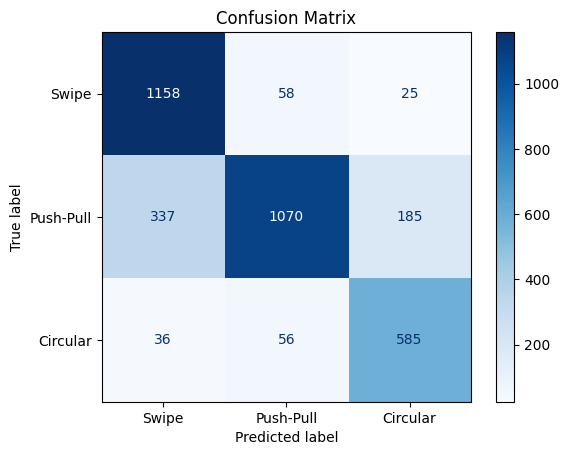
\includegraphics[width=0.45\textwidth]{figures/confusion_matrix_lr.png}
  \caption{Confusion Matrix for Logistic Regression.}
  \label{fig:confusion_matrix_lr}
\end{figure}

Logistic Regression struggled with certain gestures, such as Circular, which exhibited lower precision and F1-scores, indicating challenges in capturing complex patterns.

\subsection{Random Forest Classifier}

The Random Forest classifier, leveraging ensemble learning, achieved consistently high performance.

\begin{table}[h]
\small
\begin{center}
\caption{Performance Metrics for Random Forest Classifier}
\vspace{0.1cm}
\setlength{\tabcolsep}{+3.3mm}{
\begin{tabular}{|l|l|l|l|l|}
\hline
\textbf{Gesture} & \textbf{Precision} & \textbf{Recall} & \textbf{F1 Score} & \textbf{Support} \\ \hline
Swipe            & 0.87               & 0.95            & 0.91              & 1241             \\ \hline
Push-Pull        & 0.95               & 0.89            & 0.92              & 1592             \\ \hline
Circular         & 0.96               & 0.93            & 0.95              & 677              \\ \hline
\end{tabular}}
\end{center}
\end{table}

\begin{figure}[h]
  \centering
  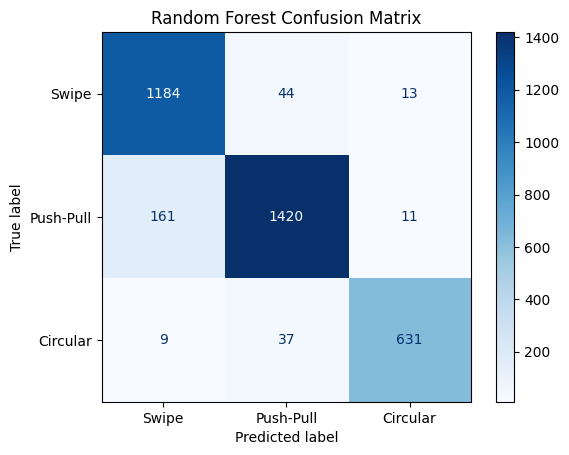
\includegraphics[width=0.45\textwidth]{figures/confusion_matrix_rf.png}
  \caption{Confusion Matrix for Random Forest Classifier.}
  \label{fig:confusion_matrix_rf}
\end{figure}

Random Forest outperformed Logistic Regression, particularly for Circular gestures, due to its ability to handle complex, non-linear relationships.

\subsection{Support Vector Machine (SVM)}

SVM with an RBF kernel effectively handled the non-linear relationships in the dataset.

\begin{table}[h]
\small
\begin{center}
\caption{Performance Metrics for Support Vector Machine}
\vspace{0.1cm}
\setlength{\tabcolsep}{+3.3mm}{
\begin{tabular}{|l|l|l|l|l|}
\hline
\textbf{Gesture} & \textbf{Precision} & \textbf{Recall} & \textbf{F1 Score} & \textbf{Support} \\ \hline
Swipe            & 0.73               & 0.97            & 0.84              & 1241             \\ \hline
Push-Pull        & 0.96               & 0.76            & 0.84              & 1592             \\ \hline
Circular         & 0.97               & 0.88            & 0.92              & 677              \\ \hline
\end{tabular}}
\end{center}
\end{table}

\begin{figure}[h]
  \centering
  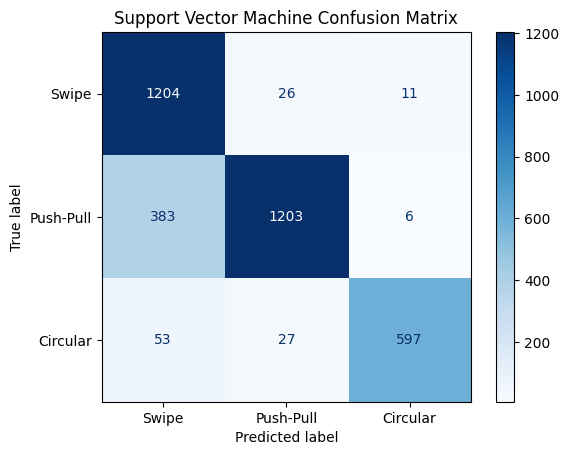
\includegraphics[width=0.45\textwidth]{figures/confusion_matrix_svm.png}
  \caption{Confusion Matrix for Support Vector Machine.}
  \label{fig:confusion_matrix_svm}
\end{figure}

Support Vector Machine demonstrated strong performance for Swipe and Circular gestures but exhibited challenges with Push-Pull gestures, as indicated by lower recall values.

\subsection{Gradient Boosted Decision Trees (XGBoost)}

XGBoost excelled in capturing non-linear relationships in the data using its gradient boosting mechanism.

\begin{table}[h]
\small
\begin{center}
\caption{Performance Metrics for XGBoost}
\vspace{0.1cm}
\setlength{\tabcolsep}{+3.3mm}{
\begin{tabular}{|l|l|l|l|l|}
\hline
\textbf{Gesture} & \textbf{Precision} & \textbf{Recall} & \textbf{F1 Score} & \textbf{Support} \\ \hline
Swipe            & 0.86               & 0.95            & 0.90              & 1241             \\ \hline
Push-Pull        & 0.90               & 0.88            & 0.89              & 1592             \\ \hline
Circular         & 0.98               & 0.87            & 0.92              & 677              \\ \hline
\end{tabular}}
\end{center}
\end{table}

\begin{figure}[h]
  \centering
  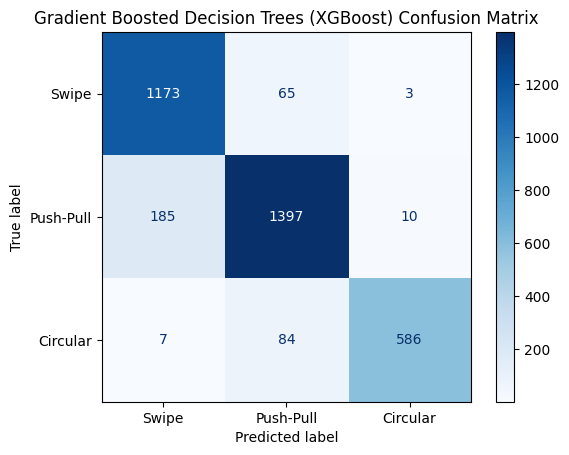
\includegraphics[width=0.45\textwidth]{figures/confusion_matrix_xgb.png}
  \caption{Confusion Matrix for XGBoost.}
  \label{fig:confusion_matrix_xgb}
\end{figure}

XGBoost offered competitive performance, particularly for Push-Pull gestures, and demonstrated balanced precision and recall across all gestures.

\subsection{Stacking Ensemble}

The stacking ensemble combined multiple classifiers, producing reliable predictions.

\begin{table}[h]
\small
\begin{center}
\caption{Performance Metrics for Stacking Ensemble}
\vspace{0.1cm}
\setlength{\tabcolsep}{+3.3mm}{
\begin{tabular}{|l|l|l|l|l|}
\hline
\textbf{Gesture} & \textbf{Precision} & \textbf{Recall} & \textbf{F1 Score} & \textbf{Support} \\ \hline
Swipe            & 0.88               & 0.94            & 0.91              & 1241             \\ \hline
Push-Pull        & 0.94               & 0.90            & 0.92              & 1592             \\ \hline
Circular         & 0.96               & 0.94            & 0.95              & 677              \\ \hline
\end{tabular}}
\end{center}
\end{table}

\begin{figure}[h]
  \centering
  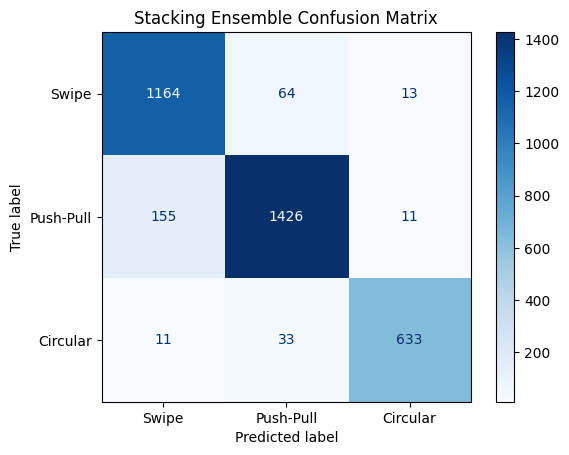
\includegraphics[width=0.45\textwidth]{figures/confusion_matrix_stacking.png}
  \caption{Confusion Matrix for Stacking Ensemble.}
  \label{fig:confusion_matrix_stacking}
\end{figure}

The Stacking Ensemble consistently achieved high performance across all gestures, showcasing the advantage of combining multiple classifiers.

\subsection{Simple Autoencoder}

The Simple Autoencoder was the first deep learning model tested, designed to reduce dimensionality and extract latent features.

\begin{table}[h]
\small
\begin{center}
\caption{Performance Metrics for Simple Autoencoder}
\vspace{0.1cm}
\setlength{\tabcolsep}{+3.3mm}{
\begin{tabular}{|l|l|l|l|l|}
\hline
\textbf{Gesture} & \textbf{Precision} & \textbf{Recall} & \textbf{F1 Score} & \textbf{Support} \\ \hline
Swipe            & 0.95               & 0.75            & 0.84              & 143              \\ \hline
Push-Pull        & 0.56               & 0.70            & 0.63              & 107              \\ \hline
Circular         & 0.55               & 0.57            & 0.56              & 123              \\ \hline
\end{tabular}}
\end{center}
\end{table}

\begin{figure}[h]
  \centering
  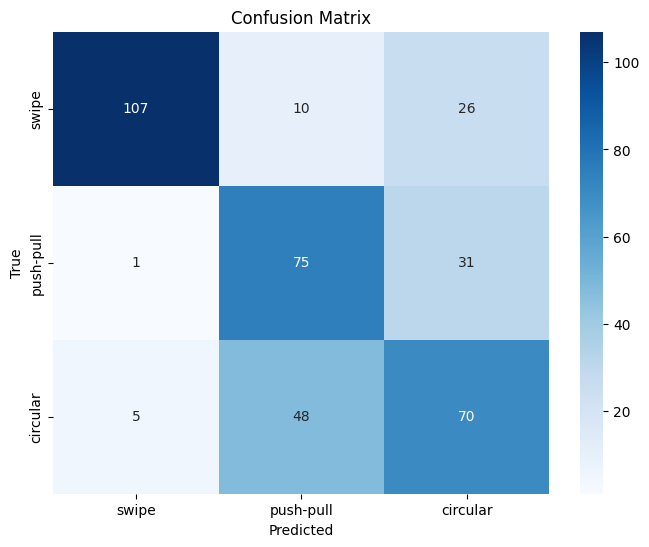
\includegraphics[width=0.45\textwidth]{figures/confusion_matrix_simple_autoencoder.png}
  \caption{Confusion Matrix for Simple Autoencoder.}
  \label{fig:confusion_matrix_simple_autoencoder}
\end{figure}

The Simple Autoencoder demonstrated a strong ability to classify the Swipe gesture but struggled with Circular gestures due to limited feature extraction.

\subsection{Autoencoder + LSTM}

The Autoencoder + LSTM model added sequential analysis capabilities, aiming to improve classification accuracy.

\begin{table}[h]
\small
\begin{center}
\caption{Performance Metrics for Autoencoder + LSTM}
\vspace{0.1cm}
\setlength{\tabcolsep}{+3.3mm}{
\begin{tabular}{|l|l|l|l|l|}
\hline
\textbf{Gesture} & \textbf{Precision} & \textbf{Recall} & \textbf{F1 Score} & \textbf{Support} \\ \hline
Swipe            & 0.92               & 0.74            & 0.82              & 143              \\ \hline
Push-Pull        & 0.61               & 0.49            & 0.54              & 107              \\ \hline
Circular         & 0.51               & 0.72            & 0.59              & 123              \\ \hline
\end{tabular}}
\end{center}
\end{table}

\begin{figure}[h]
  \centering
  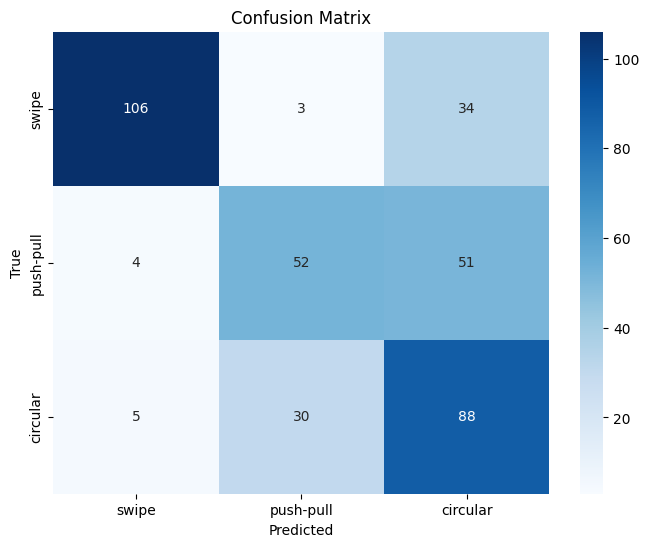
\includegraphics[width=0.45\textwidth]{figures/confusion_matrix_autoencoder_lstm.png}
  \caption{Confusion Matrix for Autoencoder + LSTM.}
  \label{fig:confusion_matrix_autoencoder_lstm}
\end{figure}

The addition of LSTM improved temporal analysis, leading to better recall for the Circular gesture but showed challenges with Push-Pull gestures.

\subsection{LSTM-Based Autoencoder}

The LSTM-Based Autoencoder utilized sequence-based encoding and decoding for feature extraction.

\begin{table}[h]
\small
\begin{center}
\caption{Performance Metrics for LSTM-Based Autoencoder}
\vspace{0.1cm}
\setlength{\tabcolsep}{+3.3mm}{
\begin{tabular}{|l|l|l|l|l|}
\hline
\textbf{Gesture} & \textbf{Precision} & \textbf{Recall} & \textbf{F1 Score} & \textbf{Support} \\ \hline
Swipe            & 0.95               & 0.71            & 0.81              & 143              \\ \hline
Push-Pull        & 0.58               & 0.62            & 0.60              & 107              \\ \hline
Circular         & 0.51               & 0.63            & 0.56              & 123              \\ \hline
\end{tabular}}
\end{center}
\end{table}

\begin{figure}[h]
  \centering
  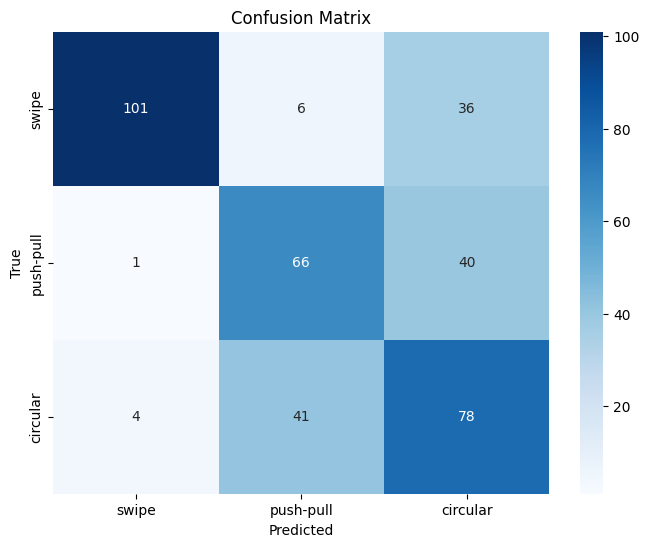
\includegraphics[width=0.45\textwidth]{figures/confusion_matrix_lstm_autoencoder.png}
  \caption{Confusion Matrix for LSTM-Based Autoencoder.}
  \label{fig:confusion_matrix_lstm_autoencoder}
\end{figure}

While the LSTM-Based Autoencoder showed competitive precision and recall for Swipe gestures, it exhibited limited improvement over simpler models for Push-Pull and Circular gestures.



\section{Discussion of Results}

This section delves into the comparative analysis of the models evaluated in this study. We discuss the strengths and weaknesses of each model in terms of accuracy, precision, recall, and F1-score across the three gestures (Swipe, Push-Pull, and Circular). Insights from confusion matrices are also highlighted to reveal areas of misclassification.

\subsection{Comparative Performance Analysis}

The evaluation of models revealed varying levels of effectiveness across the gestures. Table~\ref{tab:comparative_metrics} provides a consolidated view of key performance metrics for all models.

\begin{table*}[h]
\small
\begin{center}
\caption{Comparative Performance Metrics for All Models}
\vspace{0.1cm}
\setlength{\tabcolsep}{+2.0mm}{
\begin{tabular}{|l|l|l|l|l|}
\hline
\textbf{Model}          & \textbf{Accuracy (\%)} & \textbf{Precision} & \textbf{Recall} & \textbf{F1-Score} \\ \hline
Logistic Regression     & 80.00                 & 0.82               & 0.80            & 0.80              \\ \hline
Random Forest           & 92.17                 & 0.92               & 0.92            & 0.92              \\ \hline
Support Vector Machine  & 85.58                 & 0.88               & 0.86            & 0.86              \\ \hline
XGBoost                 & 89.91                 & 0.90               & 0.90            & 0.90              \\ \hline
Stacking Ensemble       & 91.82                 & 0.92               & 0.92            & 0.92              \\ \hline
Autoencoder             & 67.56                 & 0.71               & 0.68            & 0.68              \\ \hline
Autoencoder + LSTM      & 65.95                 & 0.70               & 0.66            & 0.67              \\ \hline
LSTM-based Autoencoder  & 65.68                 & 0.70               & 0.66            & 0.67              \\ \hline
\end{tabular}}
\label{tab:comparative_metrics}
\end{center}
\end{table*}

\subsection{Gesture-Specific Insights}

To understand model-specific behavior, we analyze performance metrics for each gesture:

\textbf{Swipe Gesture:}
\begin{itemize}
  \item Random Forest and Stacking Ensemble exhibited the best precision and recall (0.95 and 0.94, respectively).
  \item Logistic Regression struggled, with an F1-score of 0.84, primarily due to false positives in other gesture categories.
  \item Autoencoder-based models achieved moderate performance, highlighting their potential for latent feature extraction.
\end{itemize}

\textbf{Push-Pull Gesture:}
\begin{itemize}
  \item XGBoost and Stacking Ensemble models provided the most balanced performance, with F1-scores of 0.90 and 0.92, respectively.
  \item Support Vector Machine performed well but showed lower recall due to some misclassifications as Circular gestures.
  \item Autoencoder + LSTM struggled slightly, with an F1-score of 0.54, indicating room for improvement.
\end{itemize}

\textbf{Circular Gesture:}
\begin{itemize}
  \item Random Forest and Stacking Ensemble excelled, achieving F1-scores of 0.95, demonstrating their ability to correctly classify complex gesture patterns.
  \item LSTM-based Autoencoder and Autoencoder + LSTM provided competitive results but faced challenges in capturing finer distinctions.
\end{itemize}

\subsection{Confusion Matrix Analysis}

Confusion matrices provided deeper insights into model performance:
\begin{itemize}
  \item Logistic Regression struggled with the Push-Pull gesture, misclassifying many instances as Swipe.
  \item Random Forest showed balanced performance, with minimal misclassifications across all gestures.
  \item Autoencoder + LSTM and LSTM-based Autoencoder highlighted the difficulty in separating Circular and Push-Pull gestures due to overlapping RSSI patterns.
\end{itemize}

\begin{figure}[h]
  \centering
  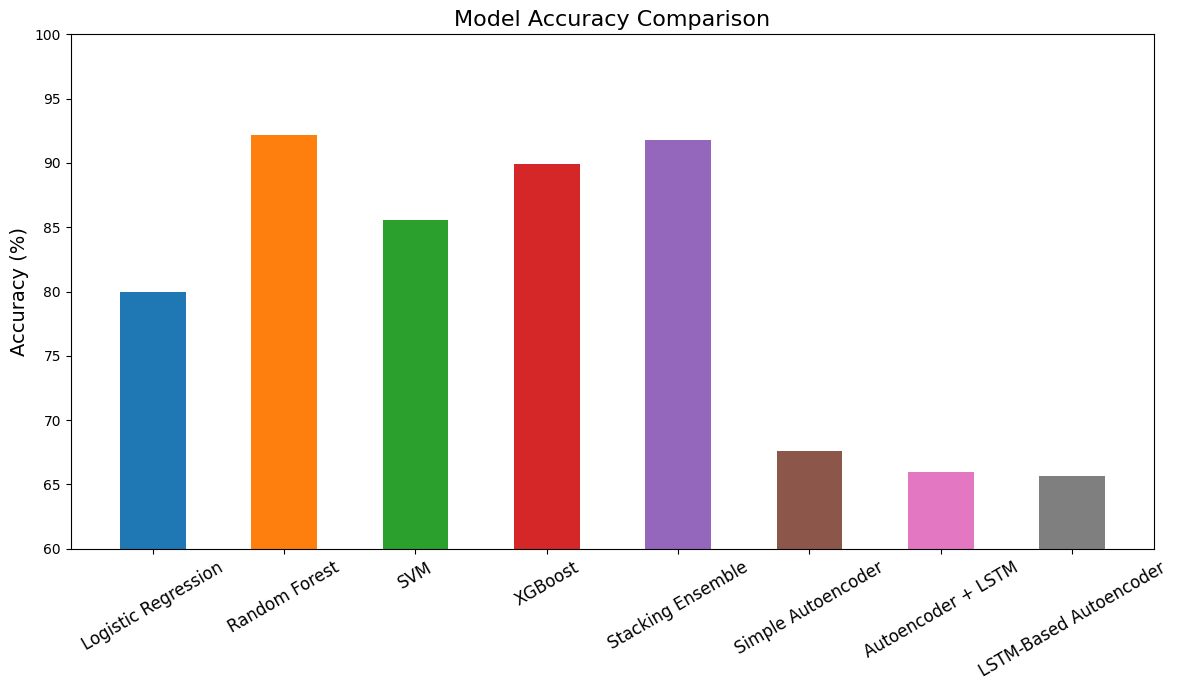
\includegraphics[width=0.45\textwidth]{figures/comparative_accuracy_chart.png}
  \caption{Comparative Accuracy Chart for All Models.}
  \label{fig:comparative_accuracy}
\end{figure}

\subsection{Key Observations}

\begin{itemize}
  \item \textbf{Model Robustness:}
    \begin{itemize}
      \item Random Forest and Stacking Ensemble consistently outperformed others, showcasing their robustness in handling varying gesture complexities.
      \item Logistic Regression, while simple, served as an effective baseline but lagged in overall performance.
      \item Autoencoder-based models showed promise for feature extraction but struggled to outperform traditional ML models.
    \end{itemize}

  \item \textbf{Performance Trade-offs:}
    \begin{itemize}
      \item Support Vector Machine demonstrated a good balance between precision and recall but was slightly overshadowed by ensemble methods.
      \item XGBoost offered competitive performance, particularly for Push-Pull gestures.
      \item Autoencoder + LSTM models provided strong latent representation capabilities but needed optimization for generalization.
    \end{itemize}

  \item \textbf{Impact of Preprocessing:}
    \begin{itemize}
      \item The 3-point moving average and interpolation during preprocessing likely enhanced the performance of ensemble models by smoothing RSSI variations and mitigating noise.
      \item Deep learning models could benefit from advanced preprocessing techniques tailored to sequential data.
    \end{itemize}
\end{itemize}

\subsection{Charts for Gesture-Level Performance}

To visually represent gesture-level performance, Figure~\ref{fig:f1_per_gesture} showcases the F1-scores for each model across all gestures.

\begin{figure}[h]
  \centering
  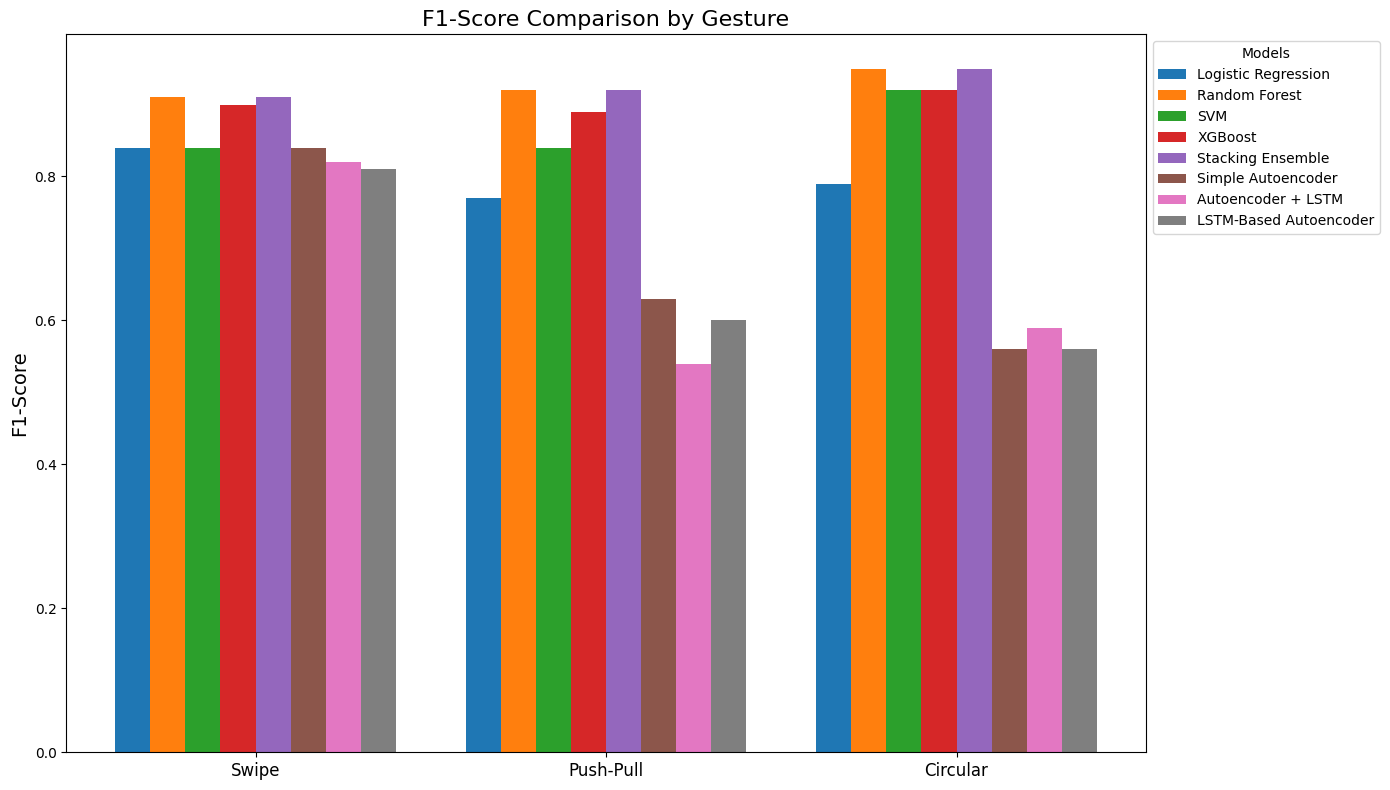
\includegraphics[width=0.45\textwidth]{figures/f1_per_gesture_chart.png}
  \caption{F1-Scores for Each Gesture Across All Models.}
  \label{fig:f1_per_gesture}
\end{figure}

\subsection{Limitations}

\begin{itemize}
  \item The dataset size was limited, which could impact generalizability.
  \item Overlapping RSSI patterns for similar gestures posed challenges for deep learning models.
  \item Autoencoder-based models showed potential but require further optimization for improved generalization and classification accuracy.
\end{itemize}

Future work will focus on expanding the dataset, optimizing deep learning architectures, and exploring advanced preprocessing methods for improved model performance.




\section{Future Directions}

The findings of this study demonstrate the feasibility and effectiveness of using Wi-Fi RSSI data for gesture recognition. However, several areas remain unexplored and provide opportunities for further research.

\subsection{Expanding the Dataset}

One of the primary limitations of this study was the relatively small dataset size. Future work could focus on:
\begin{itemize}
    \item Collecting larger and more diverse datasets under different environmental conditions, such as varying distances, obstructions, and signal interference~\cite{wang2017wifi}.
    \item Including additional gestures to expand the classification space while ensuring robust model performance~\cite{haseeb2020wisture}.
    \item Ensuring datasets capture variations due to user demographics, such as age or dominant hand, to improve model inclusivity and adaptability.
\end{itemize}

\subsection{Exploration of Advanced Models}

Although traditional machine learning models like Random Forest and ensemble methods performed well, future work could explore:
\begin{itemize}
    \item Deep learning architectures, such as Long Short-Term Memory (LSTM) networks, for capturing sequential dependencies in time-series RSSI data~\cite{haseeb2020wisture}.
    \item Hybrid models combining Convolutional Neural Networks (CNNs) for feature extraction and Recurrent Neural Networks (RNNs) for temporal pattern recognition~\cite{wang2017wifi}.
    \item Attention mechanisms to focus on critical temporal segments for gesture classification~\cite{vaswani2017attention}.
    \item Transformer-based architectures, which have shown promise in handling long-range dependencies in sequential data~\cite{vaswani2017attention}.
\end{itemize}

\subsection{Real-Time Implementation and Optimization}

Another important direction involves transitioning from offline analysis to real-time systems:
\begin{itemize}
    \item Developing lightweight models capable of running on mobile devices with limited computational resources~\cite{abdelnasser2015wifi}.
    \item Optimizing the preprocessing pipeline for on-device signal smoothing, resampling, and windowing to ensure real-time responsiveness~\cite{haseeb2020wisture}.
    \item Exploring hardware acceleration techniques, such as leveraging edge AI processors, to enhance computational efficiency.
\end{itemize}

\subsection{Generalization Across Devices}

This study focused on Wi-Fi RSSI data collected from specific devices. To improve generalization:
\begin{itemize}
    \item Investigating device-agnostic models by incorporating domain adaptation techniques to reduce performance discrepancies across different devices~\cite{wang2017wifi}.
    \item Exploring transfer learning approaches to leverage pre-trained models for new devices and environments~\cite{pan2010survey}.
    \item Conducting cross-device validation to evaluate and refine model robustness in heterogeneous hardware environments.
\end{itemize}

\subsection{Integration with Broader Systems}

Wi-Fi-based gesture recognition systems have significant potential for integration into broader applications:
\begin{itemize}
    \item Incorporating gesture recognition as part of smart home automation systems for intuitive control of IoT devices~\cite{wang2017wifi}.
    \item Exploring its use in healthcare monitoring for contactless detection of patient activities and abnormalities~\cite{abdelnasser2015wifi}.
    \item Enhancing autonomous vehicle systems by integrating Wi-Fi gesture recognition with existing sensing technologies~\cite{wang2017wifi}.
    \item Leveraging gesture recognition in interactive public displays for advertising and user engagement.
\end{itemize}

\subsection{Addressing Privacy Concerns}

Since Wi-Fi RSSI data can be sensitive, future work should consider:
\begin{itemize}
    \item Implementing privacy-preserving algorithms for data collection and processing~\cite{dwork2014algorithmic}.
    \item Studying ethical implications and ensuring compliance with data protection regulations, such as GDPR, in real-world deployments.
    \item Educating end-users about the trade-offs between functionality and privacy to foster trust and transparency.
\end{itemize}

\subsection{Incorporating Channel State Information (CSI)}

Channel State Information (CSI) provides more detailed channel-level data compared to RSSI. Future work could:
\begin{itemize}
    \item Investigate the use of CSI for improved accuracy and robustness, especially in complex environments~\cite{wang2017wifi}.
    \item Develop models capable of simultaneously utilizing RSSI and CSI to maximize gesture recognition performance~\cite{haseeb2020wisture}.
    \item Explore CSI's potential in distinguishing between gestures with subtle differences, enhancing classification granularity.
\end{itemize}

\subsection{Benchmarking and Community Contribution}

To facilitate progress in this domain:
\begin{itemize}
    \item Establishing standardized benchmarks and metrics for Wi-Fi-based gesture recognition systems~\cite{abdelnasser2015wifi}.
    \item Sharing datasets, source codes, and pre-trained models with the research community to encourage reproducibility and further innovation~\cite{haseeb2020wisture}.
    \item Creating open-source libraries to simplify the development and deployment of Wi-Fi gesture recognition applications.
\end{itemize}


\section{Conclusions}

This study has demonstrated the feasibility and effectiveness of using Wi-Fi Received Signal Strength Indicator (RSSI) data for hand gesture recognition, a contactless and hardware-agnostic approach. By leveraging advanced preprocessing techniques such as resampling, smoothing, and windowing, we transformed raw RSSI data into structured sequences suitable for machine learning models. The experimental results have shown that models like Random Forest, XGBoost, and Stacking Ensembles outperform traditional methods, achieving robust classification performance with over 90\% accuracy in most cases.

Our findings underscore the potential of Wi-Fi signals as a low-cost and ubiquitous medium for gesture recognition. Unlike Channel State Information (CSI)-based approaches, which often require specialized hardware, this study relies on standard Wi-Fi RSSI measurements, making the solution deployable on commodity devices without modifications. Furthermore, the inclusion of exploratory data analysis (EDA) revealed critical patterns in the RSSI data, providing insights into its temporal and statistical properties.

Despite the promising results, this work opens avenues for future exploration. Challenges such as scalability across diverse environments, real-time implementation, and privacy preservation remain significant. The integration of this technology into broader applications, such as smart home systems and healthcare monitoring, holds substantial promise.

By sharing our datasets and methodological framework, we aim to contribute to the growing body of research in Wi-Fi-based gesture recognition, enabling further advancements in this field. Future research can build upon this foundation, exploring innovative algorithms and applications to realize the full potential of contactless gesture recognition systems.


In conclusion, this study serves as a stepping stone for the development of accessible and scalable gesture recognition systems, demonstrating the viability of RSSI-based methods in addressing real-world challenges. We hope this work inspires further innovation in the intersection of wireless communications and human-computer interaction.

{\small
\bibliographystyle{plain}
\bibliography{egbib}
}

\end{document}
